\section{Simulation (\mmd{in progress})}
\label{sec:sim}
%%%%%%%%%%%%%%%%%%%%%%%%%%%%%%%%%%%%%%%%%%%%%%%%%%%%%%%%%%%%%%%%%%%%%%%%%%%%%%%%%%%%%%%%%%%%%%%%%%%%%%%%%%%%%%%%%%%%%%%%
To asses the sensitivity of the detector to identify an emission pattern a GEANT4 based simulation is used. 
Several emission types and the propagation of photons in the detector are simulated to produce the hit patern  
at the PMTs for each type. 
Assuming a number of test patterns of the LXe scintillation, the photons detected at the PMTs are mapped and put 
through a statistical test to check the detector's sensitivity towards those patterns.

The realistic dimension of the detector assembly is used in the simulation. The important 
geometrical and optical parameters are listed in Table~\ref{tab:OptPar}. 
The probability for a photon being transmitted/reflected at a given surface is 
determined by Fresnel's equations, which include Snell's law for the transmitted light, 
and specular reflection for the reflected light. The boundary surfaces between different media
such as, the LXe--HPFS, HPFS--vacuum and vacuum--PMT, are assumed to be perfectly smooth, 
therefore enabling only specular reflection.

%%%%%%%%%%%%%%%%%%%%%%%%%%%%%%%%%%%%%%%%%%%%%%%%%%%%%%%%%%%%%%%%%%%%%%%%%%%%%%%%%%%%%%%
\begin{table}[h]
  \centering
  \caption{The parameters used in simulation}
  \label{tab:OptPar}
  \begin{tabular}{|c c||c c|}
  \hline
  Parameter & Value & Parameter & Value \\
  \hline
  LXe absorption length & 100 cm & No. of PMT & 20\\
  %\hline
  LXe scattering length & 35 cm & PMT active area & 22mm $\times$ 22mm\\
  %\hline
  HPFS absorption length & 100 cm & PMT QE & $\geq$ 30\% \\
 % \hline
  HPFS scattering length & $\infty$ & PMT distance from centre & 39 mm\\
 % \hline
  LXe refractive index & 1.61 & LXe bubble radius & 1cm\\
  %\hline
  HPFS refractive index & 1.57 & HPFS shell thickness & 2 cm \\
  Scintillation wavelength & 178 $\pm$ 14 nm & Invar tube diameter & 1 mm\\
  \hline
 \end{tabular}
\end{table}
%%%%%%%%%%%%%%%%%%%%%%%%%%%%%%%%%%%%%%%%%%%%%%%%%%%%%%%%%%%%%%%%%%%%%%%%%%%%%%%%%%%%%%%

The photons reaching the PMTs can either be detected, absorbed or reflected from the photocathode 
or the PMT window. A simplified approach of the above possibilities is considered -- 
A photon on the PMT has 30\% probability to be detected (since QE $\geq$ 30\%), 50\% probability to get 
absorbed and 20\% probability to get specularly reflected. As the scintillation light in a particular 
event is emitted by a cloud of excited diatomic molecules, with a linear size much smaller than that 
of the optical system, each event is simulated as a number of photons that are emitted from a point 
in the LXe. The events are uniformly generated in the LXe volume to simulate an entirely radiated 
target much smaller than the mean free path length of the source particles in LXe.

For each scintillation event, a number of photons are detected by the PMTs, with a possibility of 
no photons detected by some of the PMTs. The exact position on the photocathode which the photons hit, 
and the exact number of photons falling on a PMT are not known. The electronic signal generated in a PMT 
for a certain number of incident photon is statistical in nature. The simulation is performed for both 
ideal photon counting and statistical photon counting. The R8520 PMTs also has  ~20\% probability 
for double photoelectris emission for 178 nm photons, which is also included in the simulation.
Each detected photon 
on a PMT is then assigned a uniformly random position on the PMT surface. The direction of this point with respect 
to the center of the LXe sphere is defined as the incident direction of the photon. The direction information 
is then used to calculate the angles between all possible pairs of photon in an event.

In order to test the emission pattern, the angle correlation distribution of a large sample ($10^5$ events) 
from isotropic emission is considered to be the PDF of the null hypothesis and is compared 
to that of a number of smaller samples ($10^4$ events) from different types of anisotropic emissions. 
The reduced $\chi^2$ for each sample is calculated as follows.

\begin{equation}
\chi^2/\nu = \frac{1}{\nu} \sum^{\nu}_{i=1} \frac{(O_i - E_i)^2}{E_i}
\label{redchi2}
\end{equation}

where, $O_i$ is the observed count in the $i^{th}$ angle bin, $E_i$ is the expected count in the $i^{th}$ 
angle bin and $\nu$ is the total number of angle bins which is also the degree of freedom. In this analysis, 
60 bins of identical width are used. The anisotropic emission patterns used in the analysis are listed 
in Table~\ref{tab:AnisoPattern}. For each emission pattern,  an anisotropic pattern is taken to be embedded 
in an isotropic background. The fraction of photons in the anisotropic pattern ($r_{aniso}$) is 10 \% of the net photons 
and the rest is the isotropic background. For multiple beams in a pattern $r_{aniso}$ is spitted among them 
as mentioned in the Table. The intensity of the beams of photons are of Gaussian nature, and their emission direction are 
randomly varied in each event.

%%%%%%%%%%%%%%%%%%%%%%%%%%%%%%%%%%%%%%%%%%%%%%%%%%%%%%%%%%%%%%%%%%%%%%%%%%%%%%%%%%%%%%%
\begin{table}[h]
  \centering
  \caption{Emission patterns. For all patterns $r_{aniso}$ = 0.1 from a 
  total of 50 photon/event.}
  \label{tab:AnisoPattern}
  \begin{tabular}{|c | c| c | c|}
  \hline
  Pattern no. & No. of beams and type & Beam half widths & Signal fractions \\
  %\hline
  1 & 1 & $\sigma_1$ = $5^{0}$ & $r_1$ = 1 \\
  %\hline
   2 & 1 & $\sigma_1$ = $15^{0}$ & $r_1$ = 1 \\
  %\hline
   3 & 2 correlated & $\sigma_1$ = $5^{0}$, $\sigma_2$ = $5^{0}$ & $r_1$ = 0.5, $r_2$ = 0.5  \\
  %\hline
   4 & 2 correlated & $\sigma_1$ = $15^{0}$, $\sigma_2$ = $15^{0}$ & $r_1$ = 0.5, $r_2$ = 0.5 \\
  %\hline
   5 & 2 correlated & $\sigma_1$ = $5^{0}$, $\sigma_2$ = $10^{0}$ & $r_1$ = 0.5, $r_2$ = 0.5 \\
  %\hline
   6 & 2 correlated & $\sigma_1$ = $30^{0}$, $\sigma_2$ = $10^{0}$ & $r_1$ = 0.5, $r_2$ = 0.5 \\
  %\hline
   7 & 2 correlated & $\sigma_1$ = $5^{0}$, $\sigma_2$ = $5^{0}$ & $r_1$ = 0.5, $r_2$ = 0.5 \\
  %\hline
   8 & 2 correlated & $\sigma_1$ = $15^{0}$, $\sigma_2$ = $15^{0}$ & $r_1$ = 0.5, $r_2$ = 0.5 \\
  %\hline
   9 & 2 correlated & $\sigma_1$ = $10^{0}$, $\sigma_2$ = $30^{0}$ & $r_1$ = 0.2, $r_2$ = 0.8 \\
  %\hline
    10 & 2 correlated & $\sigma_1$ = $30^{0}$, $\sigma_2$ = $10^{0}$ & $r_1$ = 0.2, $r_2$ = 0.8 \\
  \hline
 \end{tabular}
\end{table}
%%%%%%%%%%%%%%%%%%%%%%%%%%%%%%%%%%%%%%%%%%%%%%%%%%%%%%%%%%%%%%%%%%%%%%%%%%%%%%%%%%%%%%%

Results:

%%%%%%%%%%%%%%%%%%%%%%%%%%%%%%%%%%%%%%%%%%%%%%%%%%%%%%%%%%%%%%%%%%%%%%%%%
\begin{figure}[h]
\centerline{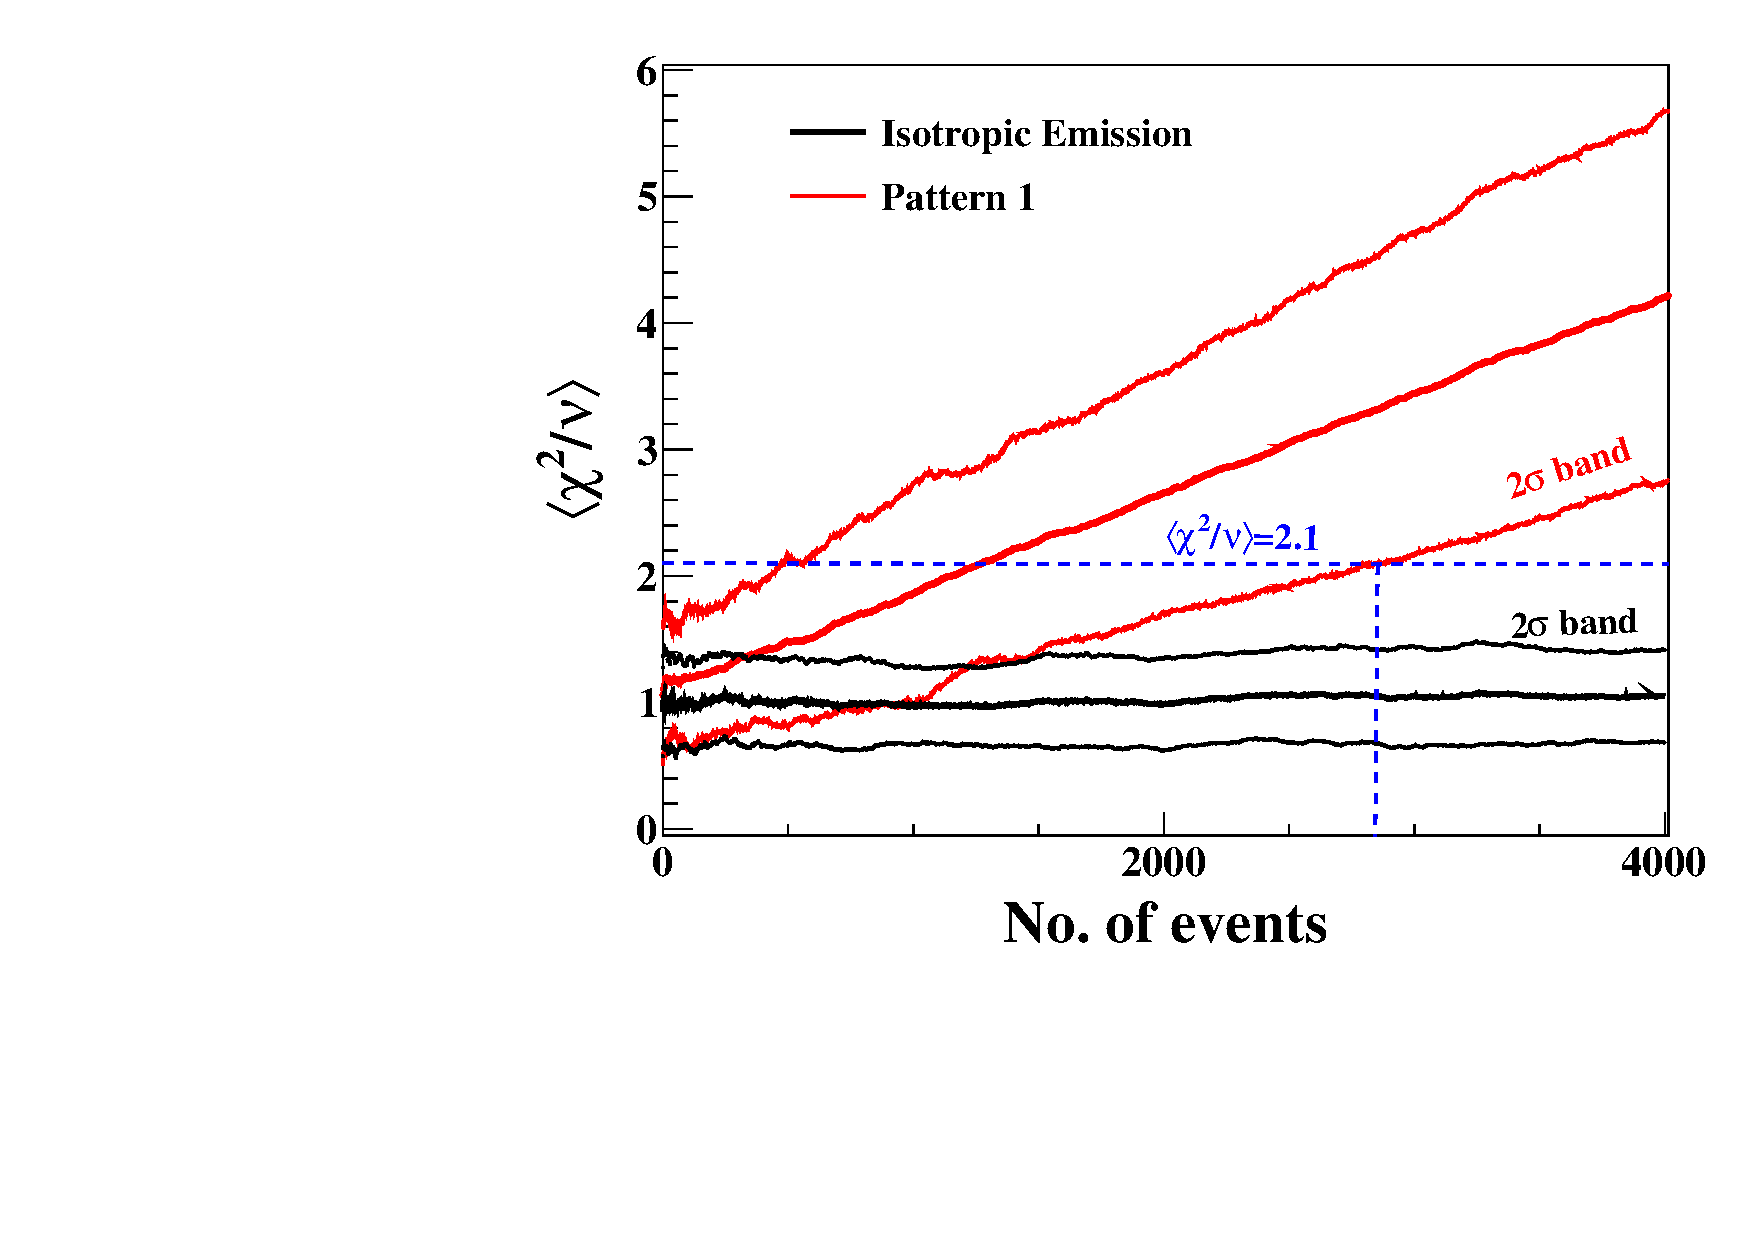
\includegraphics[width=0.5\linewidth]{Pattern1.pdf}}
\caption{}
\label{fig:pattern1}
\end{figure}
%%%%%%%%%%%%%%%%%%%%%%%%%%%%%%%%%%%%%%%%%%%%%%%%%%%%%%%%%%%%%%%%%%%%%%%%%%%%
